\section{Materiales y métodos}

En esta sección serán expuestos las diferentes herramientas y métodos utilizados para llevar a cabo el proyecto, así como los resultados obtenidos con cada una de ellas.

\subsection{Materiales}
\subsubsection{Human Phenotype Ontology}

La \textbf{Human Phenotype Ontology (HPO)} es un proyecto que desarrolla un vocabulario estandarizado y jerárquico para describir fenotipos humanos, con el objetivo de apoyar el diagnóstico y la investigación de enfermedades genéticas. Además de definir y organizar características fenotípicas específicas, la HPO permite identificar los genes y variantes genéticas asociadas a cada fenotipo, de esta manera facilita el análisis de correlaciones genotipo-fenotipo a los usuarios.

\subsubsection{STRING}

\textbf{STRING} es una base de datos que integra distintas fuentes de información y que además permite analizar y visualizar interacciones entre proteínas y genes. Pueden ser de dos tipos: interacciones físicas o interacciones funcionales. Las interacciones físicas permiten identificar compatibilidades y relaciones, mientras que las funcionales determinan si dos o más proteínas son compatibles aún sin tener interacción directa. Así pues, se pueden realizar perfiles filogenéticos y conocer genes con patrones similares, además de aportar información sobre patrones moleculares, mapas bioquímicos y mejorar la compresión de los sistemas biológicos.

\subsubsection{Python}
\textbf{Python} es uno de los lenguajes de programación más usados del mundo. Se trata de un lenguaje de alto nivel con una sintaxis sencilla y fácil de entender que dispone de multitud de paquetes de código abierto. Se caracteriza por ser interpretado, es decir, no se requiere de compilación previa a instrucciones de lenguaje máquina ya que se emplea un entorno o intérprete para ejecutar el código. La versión utilizada en este proyecto es ?.

\subsubsection{R}
\textbf{R} es otro de los lenguajes de programación más importantes en el campo de la estadística. Es un entorno de software libre y también es un lenguaje interpretado. A diferencia de otros softwares de análisis de datos, R tiene un entorno completamente integrado y coherente. Proporciona una amplia gama de técnicas estadísticas y gráficas. La versión utilizada en este proyecto es ?.

\subsubsection{iGraph}
\textbf{iGraph} es una biblioteca de código abierto utilizada para el análisis y visualización de redes complejas. Es una herramienta muy útil para el estudio de los sistemas biológicos ya que estos están compuestos por genes, moléculas, proteínas, etc, que interactúan formando grafos complejos de analizar a simple vista. Está implementado en C, aunque también puede ser utilizado en otros lenguajes como R y Python. 

Esta herramienta presenta muchas ventajas, entre las que destacamos: la integración de todo tipo de datos ómicos, la visualización de datos de forma interactiva, mejora la comprensión de las relaciones entre las distintas biomoléculas del sistema, permite la identificación de nodos clave en la red biológica, facilita el descubrimiento de grupos funcionales de genes o proteínas y predice cómo ciertas modificaciones podrían perturbar los sistemas.

\subsubsection{Pandas}
\textbf{Pandas} se trata de una popular librería de Python de código abierto muy necesaria para el ámbito de Data Science y Machine Learning. Proporciona unas estructuras poderosas y flexibles implementando todas las herramientas necesarias para el análisis de datos, ya que permite la carga, modelado, análisis, manipulación y preparación de datos.

\subsubsection{Algoritmos de clusterización}
En el presente proyecto, uno de los objetivos es la identificación de patrones entre los distintos genes asociados al fenotipo de la aniridia. Para ello, es necesario el agrupamiento de aquellas biomoléculas con mayor similitud dentro nuestra red biológica, así que se aplicarán algoritmos nos permitan detectar estructuras sin necesidad de tener conocimiento previo. Vamos a hablar de los algoritmos de Givan-Newman, de optimización voraz, de propagación de etiquetas y de Louvain.

Primero, tenemos el \textbf{algoritmo de Givan-Newman}, que es uno de los métodos más utilizados para la detección de comunidades dentro de sistemas complejos de datos. Su funcionamiento se basa en eliminar progresivamente aquellos enlaces que conectan grupos de nodos con mayor densidad dentro de la red, para visualizar finalmente subgrafos desconectados que representan las comunidades.

Por otra parte, el \textbf{algoritmo de optimización voraz} es un algoritmo que dado un problema, elige aquellas decisiones localmente óptimas con el propósito de encontrar la solución más óptima globalmente. A medida que va tomando unas decisiones, el algoritmo no reconsidera ningún paso ya realizado.

Además, el \textbf{algoritmo de propagación de etiquetas} es una técnica que nos permite encontrar comunidades dentro del sistema velozmente. El funcionamiento se basa en la asignación de etiquetas a nodos, que en cada iteración se van propagando por la red y converge finalmente cuando cada nodo posee la etiqueta perteceneciente a su vecino más cercano. Una de las ventajas de este algoritmo es que no es necesaria la predefinición de un número de clústers.

Por último, el \textbf{algoritmo de Louvain} se basa en el concepto de modularidad, es decir, tiene como objetivo maximizar el número de aristas dentro de una comunidad y minimizar el número de relaciones entre distintas comunidades. Este algoritmo es muy recomendable para sistemas biológicos muy amplios, ya que se obtienen comunidades compactas y bien definidas.

\subsubsection{Otras librerías empleadas}

\subsubsection{Software empleado para la generación de diagramas}

\subsubsection{GitHub?}

\vspace{3pt}
\subsection{Métodos}
BORRADOR:
*OPCIÓN 1*
Para realizar este estudio, el primer paso que se llevó a cabo fue la obtención de los genes relacionados con el fenotipo. Los descargamos de la página Human Phenotype Ontology mediante la introducción del ID del fenotipo, en nuestro caso "HP:0000526". Una vez obtenidos los genes, realizamos una red de interacción de los genes asociados a nuestro fenotipo mediante la herramienta STRINGDB.

A continuación, se muestran los pasos llevados a cabo para obtener una red de interacción de los genes de un fenotipo concreto:

\begin{itemize}
	\item Visitamos la página de STRING
	\item Seleccionamos la opción para intnroducir múltiples proteínas
	\item Introducimos solo los nombres de los genes descargados de Human Phenotype Ontology.
	\item Especificamos la especie, en este caso, Homo sapiens.
	\item STRING generará una red de interacciones, mostrando conexiones basadas en interacciones experimentales, predicciones y bases de datos de coexpresión.
	\item Se guarda como imagen la red obtenida.
\end{itemize}

Entre los objetivos del uso de STRING están visualizar las interacciones proteicas conocidas y predichas, identificar posibles proteínas clave o "hubs" dentro de la red y evaluar la conectividad y la funcionalidad de los genes en el contexto del fenotipo elegido.

Tras introducir el nombre de todos los genes asociados a nuestro fenotipo obtuvimos la siguiente red de interacciones:

\newpage

\begin{figure}[h] % [h] indica que queremos la imagen aquí, en la posición actual
	\centering
	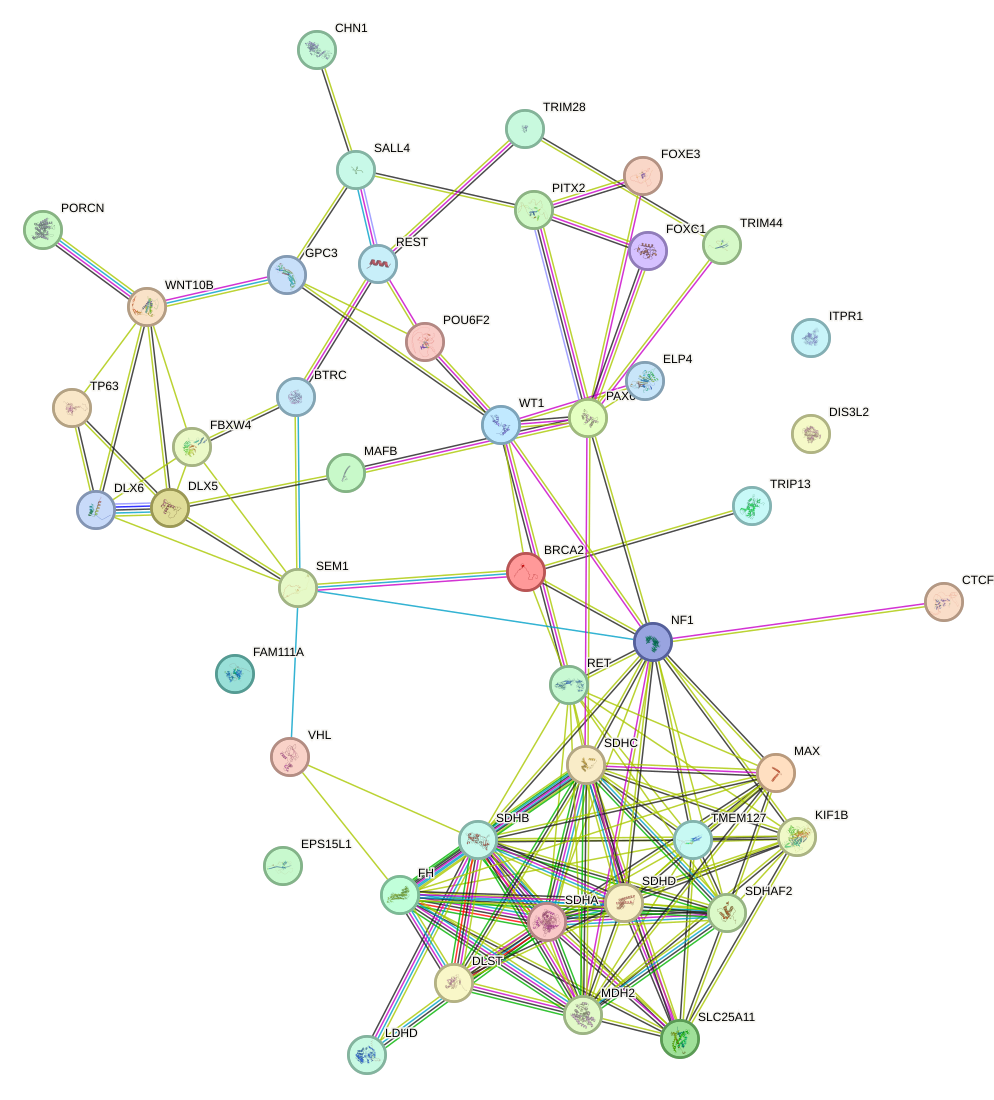
\includegraphics[width=1\textwidth]{figures/red_interaccion_aniridia.png} % Especifica la ruta y el tamaño
	\caption{Red de interacción con los genes asociados al fenotipo HP:0000526} % Agrega una leyenda si deseas
	\label{fig:mi-imagen} % Etiqueta para referenciar la imagen en el texto
\end{figure}

*OPCIÓN 2*
Para la identificación de genes asociados a la aniridia, implementamos una función en Python que hace uso de la API de Human Phenotype Ontology (HPO). Esta función recibe como parámetro el código HPO del fenotipo de interés, en este caso la aniridia, cuyo código es HP:0000526. Con este código realiza una solicitud GET a la API de HPO para recuperar información sobre los genes asociados. Si la respuesta es satisfactoria (código de estado 200), extrae y devuelve la lista de genes vinculados al fenotipo. En caso contrario, se imprime un mensaje de error y se devuelve una lista vacía.

Posteriormente, construimos una URL utilizando los símbolos de los genes obtenidos, para hacer una solicitud GET a la API de StringDB. Esta API proporciona datos sobre interacciones de proteínas. La solicitud devuelve una red de interacciones de proteínas, la cual almacenamos en la imagen .
También analizamos y filtramos los resultados de enriquecimiento en categorías relevantes. Las búsquedas específicas en estos resultados de enfermedades y genes se realizan mediante palabras clave y patrones relevantes, y los resultados se guardan en archivos CSV para facilitar su análisis posterior.

Finalmente, descargamos la red de interacciones en formato TSV usando otra solicitud GET a la API de StringDB. Si la descarga es exitosa, el archivo se guarda con el nombre de archivo especificado o, en caso contrario, con el nombre predeterminado reddescargada.tsv. Ante cualquier error en la descarga, se imprime un mensaje de advertencia.

Al cargar el archivo TSV descargado, seleccionamos las columnas de nombres preferidos y eliminamos las filas duplicadas. Estos datos se guardan en un archivo de texto llamado genesigraph.txt, que contiene únicamente los nombres de los genes relevantes para un análisis adicional de la red biológica.

\subsubsection{Flujo de trabajo}

\newpage

\section{Tipo de metodología}

En esta sección se describe la metodología detallada para el análisis de redes génicas en el contexto de la aniridia, empleando el algoritmo DIAMOnD (Disease Module Detection) y técnicas de clustering para identificar genes asociados funcionalmente con PAX6. El objetivo de este análisis es comprender cómo las interacciones entre estos genes pueden influir en la manifestación clínica de la aniridia y en su relación con otros trastornos sistémicos.

\subsection{Construcción de la red de interacciones génicas}

\subsubsection{Obtención de Datos de Interacción Génica}

Se recopilaron datos de interacción génica a partir de STRINGdb (v11.5) para construir una red basada en las interacciones conocidas de PAX6 y otros genes asociados a la aniridia. La base de datos STRINGdb proporciona un puntaje de confiabilidad para cada interacción basado en evidencia experimental, coexpresión, bases de datos de conocimiento, y otros criterios. Para garantizar la relevancia biológica en el contexto de la aniridia, solo se seleccionaron interacciones con un puntaje de confianza superior a 0.7 (umbral que indica alta probabilidad de interacción funcional).

\subsubsection{Construcción de la Red Inicial}

A partir de los datos obtenidos, se construyó una red de interacciones en Python utilizando la librería NetworkX. En esta red, los nodos representan genes y las aristas indican interacciones funcionales entre ellos. Los genes de interés fueron seleccionados como puntos de partida o "semillas" para el análisis de módulos funcionales. Estos incluyeron no solo a PAX6, sino también genes que, de acuerdo con estudios previos, tienen relevancia funcional en la aniridia, como FOXC1, WT1, COL4A1 y PITX2. Estos genes semilla fueron elegidos en base a su relación funcional conocida con PAX6 y su implicación en el desarrollo ocular y otras funciones biológicas relevantes para la patología.

\subsection{Aplicación del Algoritmo DIAMOnD para la Identificación de Módulos de Enfermedad}
\subsubsection{Implementación del Algoritmo DIAMOnD}

El análisis del módulo de enfermedad se llevó a cabo mediante la implementación del algoritmo DIAMOnD (Disease Module Detection) en la red génica construida. DIAMOnD fue diseñado para detectar módulos de enfermedad mediante la expansión progresiva de un conjunto de genes basado en la conectividad. Este algoritmo prioriza aquellos genes que muestran mayor número de conexiones hacia el módulo de interés, permitiendo identificar aquellos que, aunque no están directamente implicados en la patología, poseen relaciones funcionales clave.

\subsubsection{Parámetros de Configuración en DIAMOnD}

El algoritmo se configuró para comenzar con los genes semilla seleccionados (PAX6, FOXC1, WT1, COL4A1, y PITX2) y expandir el módulo añadiendo genes en iteraciones. En cada iteración, se evalúan los genes adyacentes a los genes del módulo existente, y se priorizan aquellos con el mayor número de conexiones (o "vecinos") hacia los genes en el módulo. Este proceso se repite hasta alcanzar un tamaño predefinido para el módulo o hasta que se agoten los genes candidatos que cumplen con el criterio de conectividad.

\subsubsection{Resultados de la Expansión del Módulo}

Al finalizar las iteraciones, se obtiene un módulo expandido de genes que presentan una posible relación funcional con la aniridia. Este módulo incluye no solo los genes semilla, sino también genes adicionales con alta conectividad hacia estos y que podrían estar implicados en vías y funciones relevantes para la patología. Los genes identificados en este módulo se consideran candidatos para un análisis posterior de funciones y vías.

\subsection{Análisis de Clustering para la Identificación de Submódulos Funcionales}
\subsubsection{Aplicación de Clustering en el Módulo Expandido}

Para analizar la estructura interna del módulo expandido, se aplicaron técnicas de clustering en la red de genes seleccionados. Se utilizó el método de clustering jerárquico (enfoque de Ben-Dor et al., 1999) para identificar subgrupos dentro del módulo. Este enfoque permite agrupar genes en función de su similitud de conectividad y su co-ocurrencia en rutas biológicas. El clustering jerárquico es especialmente útil para identificar genes que, aunque puedan estar en el mismo módulo, desempeñan roles en funciones o rutas específicas.

\subsubsection{Interpretación de los Clusters}

Cada cluster resultante fue interpretado en función de las funciones y vías asociadas a los genes incluidos. Este análisis permite observar si ciertos grupos de genes comparten funciones específicas o están involucrados en vías biológicas que podrían contribuir a la patología de la aniridia. Los clusters identificados se utilizan como base para el análisis de enriquecimiento funcional descrito a continuación.

\subsection{Análisis de Enriquecimiento Funcional de los Clusters}
\subsubsection{Herramientas y Procedimiento para el Enriquecimiento Funcional}

El análisis de enriquecimiento funcional se llevó a cabo utilizando GOATOOLS y Enrichr, herramientas que permiten realizar análisis de sobre-representación de términos del Gene Ontology (GO) y otras bases de datos de rutas y procesos biológicos. En este análisis, se seleccionaron las categorías de procesos biológicos, funciones moleculares y componentes celulares, permitiendo observar qué términos están significativamente sobre-representados en cada cluster.

\subsubsection{Identificación de Funciones y Vías Clave}

Se calcularon p-valores ajustados mediante el método de FDR (False Discovery Rate) para los términos enriquecidos, considerando significativos aquellos con valores inferiores a 0.05. Este análisis permite identificar procesos y vías específicas en las que los genes del módulo están implicados, lo cual es esencial para entender cómo la disfunción en estas interacciones contribuye a la presentación clínica de la aniridia. En particular, el análisis se enfocó en vías de desarrollo ocular, rutas de señalización y procesos morfogenéticos.

\subsection{Validación de los Resultados y Control de Calidad}
\subsubsection{Validación con Estudios Previos y Datos Experimentales}

Los resultados obtenidos se compararon con la literatura y datos previos sobre PAX6 y genes asociados. Los genes y las funciones identificadas en el análisis de DIAMOnD y de enriquecimiento funcional fueron cotejados con estudios experimentales previos para validar su relevancia en el contexto de la aniridia. Esta etapa de validación es crucial para confirmar que los genes incluidos en el módulo son relevantes y para reducir falsos positivos en el análisis.

\subsubsection{Control de Calidad y Ajuste de Parámetros}

Se realizaron análisis de sensibilidad ajustando parámetros clave, como el puntaje de interacción de STRINGdb y el tamaño del módulo, para evaluar la robustez de los resultados. Se examinó el efecto de estos ajustes en la composición del módulo y en los términos de enriquecimiento funcional, asegurando así que los resultados sean consistentes y representativos.